\section{LLM-Inference-Bench}
{{\footnotesize
\begin{description}[labelwidth=5em, labelsep=1em, leftmargin=*, align=left, itemsep=0.3em, parsep=0em]
  \item[date:] 2024-10-31
  \item[version:] TODO
  \item[last\_updated:] 2024-11
  \item[expired:] unknown
  \item[valid:] yes
  \item[valid\_date:] TODO
  \item[url:] \href{https://github.com/argonne-lcf/LLM-Inference-Bench}{https://github.com/argonne-lcf/LLM-Inference-Bench}
  \item[doi:] TODO
  \item[domain:] LLM; HPC/inference
  \item[focus:] Hardware performance benchmarking of LLMs on AI accelerators
  \item[keywords:]
    - LLM
    - inference benchmarking
    - GPU
    - accelerator
    - throughput
  \item[summary:] A suite evaluating inference performance of LLMs (LLaMA, Mistral, Qwen) across diverse accelerators (NVIDIA, AMD, Intel, SambaNova) and frameworks (vLLM, DeepSpeed-MII, etc.), with an interactive dashboard and per-platform metrics. :contentReference[oaicite:3]\{index=3\}

  \item[licensing:] TODO
  \item[task\_types:]
    - Inference Benchmarking
  \item[ai\_capability\_measured:]
    - Inference throughput
    - latency
    - hardware utilization
  \item[metrics:]
    - Token throughput (tok/s)
    - Latency
    - Framework-hardware mix performance
  \item[models:]
    - LLaMA-2-7B
    - LLaMA-2-70B
    - Mistral-7B
    - Qwen-7B
  \item[ml\_motif:]
    - HPC/inference
  \item[type:] Dataset
  \item[ml\_task:]
    - Inference Benchmarking
  \item[solutions:] TODO
  \item[notes:] Licensed under BSD-3, maintained by Argonne; supports GPUs and accelerators. :contentReference[oaicite:4]\{index=4\}

  \item[contact.name:] Krishna Teja Chitty-Venkata (Argonne LCF)
  \item[contact.email:] unknown
  \item[results.links.name:] ChatGPT LLM
  \item[fair.reproducible:] Yes
  \item[fair.benchmark\_ready:] Yes
  \item[ratings.software.rating:] 0
  \item[ratings.software.reason:] Not analyzed.

  \item[ratings.specification.rating:] 9.0
  \item[ratings.specification.reason:] PDE tasks (forward/inverse) and I/O structures are clearly specified with detailed PDE context and constraints.

  \item[ratings.dataset.rating:] 10.0
  \item[ratings.dataset.reason:] Hosted via DaRUS with a DOI, well-documented, versioned, and FAIR-compliant.

  \item[ratings.metrics.rating:] 9.0
  \item[ratings.metrics.reason:] Uses RMSE variants and Fourier-based errors.

  \item[ratings.reference\_solution.rating:] 10.0
  \item[ratings.reference\_solution.reason:] Baselines (FNO, U-Net, PINN) implemented and ready-to-run; strong community adoption.

  \item[ratings.documentation.rating:] 9.0
  \item[ratings.documentation.reason:] Clean GitHub with usage, dataset links, and tutorial notebooks.

  \item[id:] llm-inference-bench
  \item[Citations:] \cite{10820566}
  \item[Ratings:]
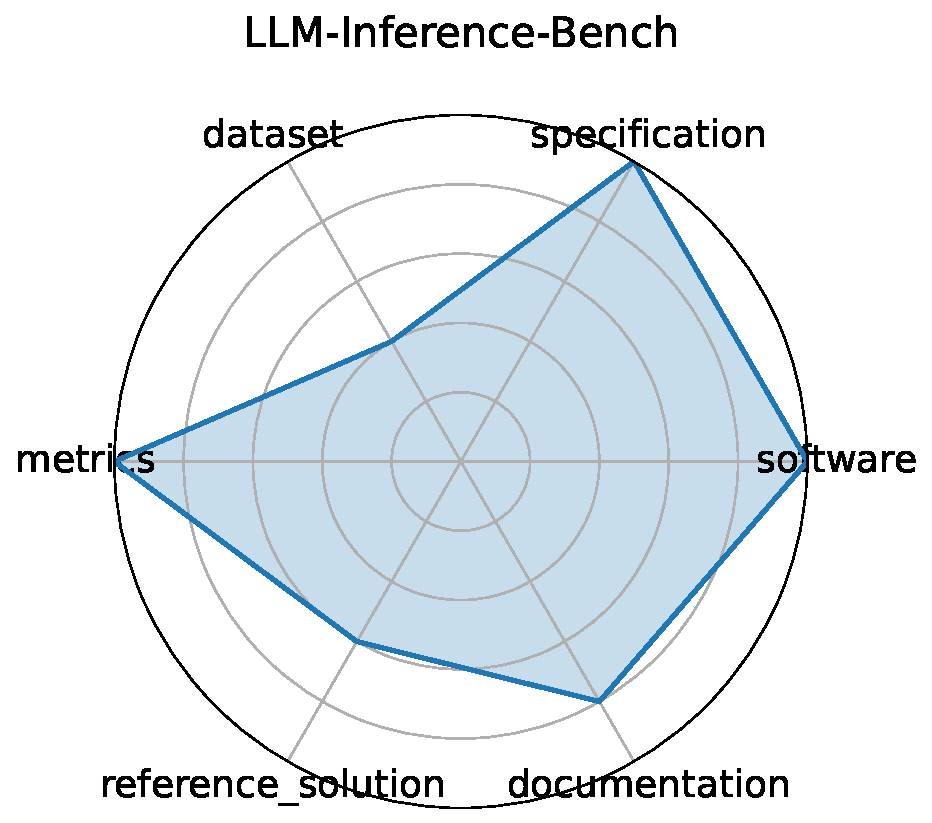
\includegraphics[width=0.2\textwidth]{llm-inference-bench_radar.pdf}
\end{description}
}}
\clearpage